\documentclass[aspectratio=169]{beamer}
\usetheme{metropolis}
%\usecolortheme{owl}
\usecolortheme[snowy]{owl}
\metroset{block=fill}

\usepackage{appendixnumberbeamer}
\usepackage{booktabs}
\usepackage{hyperref}
\usepackage{fancyvrb}
\usepackage{xcolor}
\usepackage{makecell}
\hypersetup{colorlinks,allcolors=.,urlcolor=blue}

\title{Linux Kernel ProCamp}
\subtitle{Presentation}
%\date{\today}
\author{Sam Protsenko \\ Senior Software Engineer, Linux Kernel ProCamp Trainer}
\date{\vspace*{5mm}August 28, 2019}
\institute{GlobalLogic}

\begin{document}

\maketitle

%\begin{frame}{Agenda}
%  \setbeamertemplate{section in toc}[sections numbered]
%  \tableofcontents[hideallsubsections]
%\end{frame}

\section{Linux Usages}

\begin{frame}
  \frametitle{Linux Usages: Non-Embedded}
  \begin{columns}
    \column{0.5\textwidth}
    Non-embedded systems:
      \begin{itemize}
        \item Servers
        \item Desktops
        \item Supercomputers
      \end{itemize}
    \column{0.5\textwidth}
    \begin{figure}
      \centering
      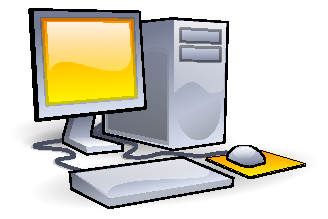
\includegraphics[scale=0.7]{images/pc.pdf}
      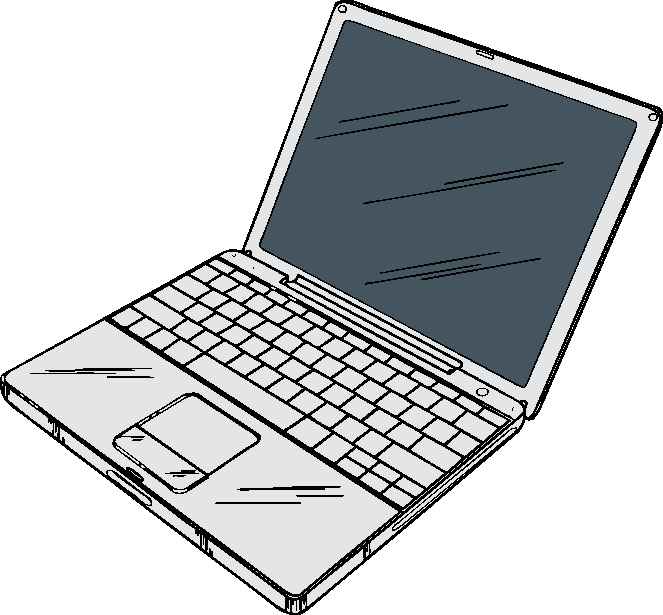
\includegraphics[scale=0.25]{images/laptop.pdf}
      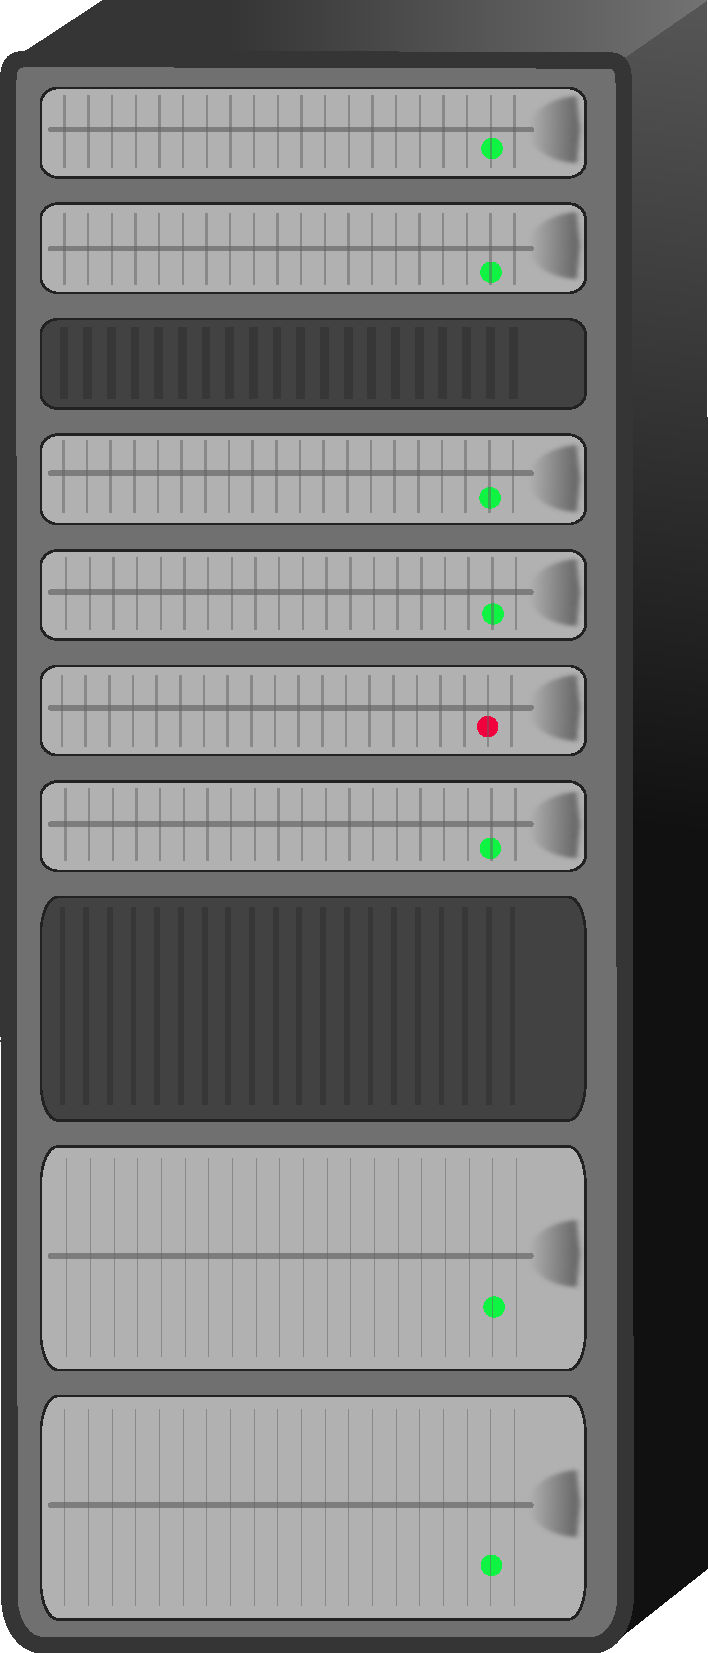
\includegraphics[scale=0.10]{images/server.pdf}
      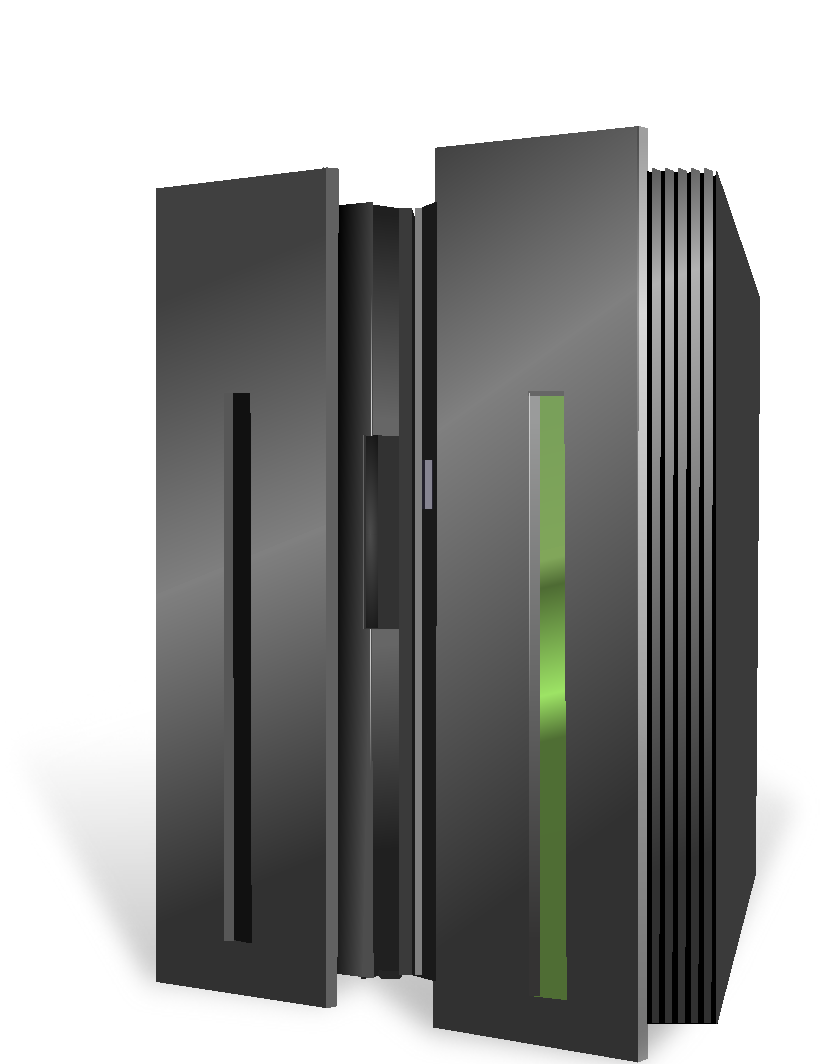
\includegraphics[scale=0.2]{images/supercomputer.pdf}
    \end{figure}
  \end{columns}
\end{frame}

\begin{frame}
  \frametitle{Linux Usages: Embedded}
  \begin{columns}
    \column{0.35\textwidth}
    Embedded Systems:
     \begin{itemize}
       \item Mobile
       \item Automotive
       \item Networking
       \item Smart TVs, game consoles, set-top boxes
       \item IoT
       \item Medical
       \item Aerospace
       \item Industry
     \end{itemize}
    \column{0.65\textwidth}
    \begin{figure}
      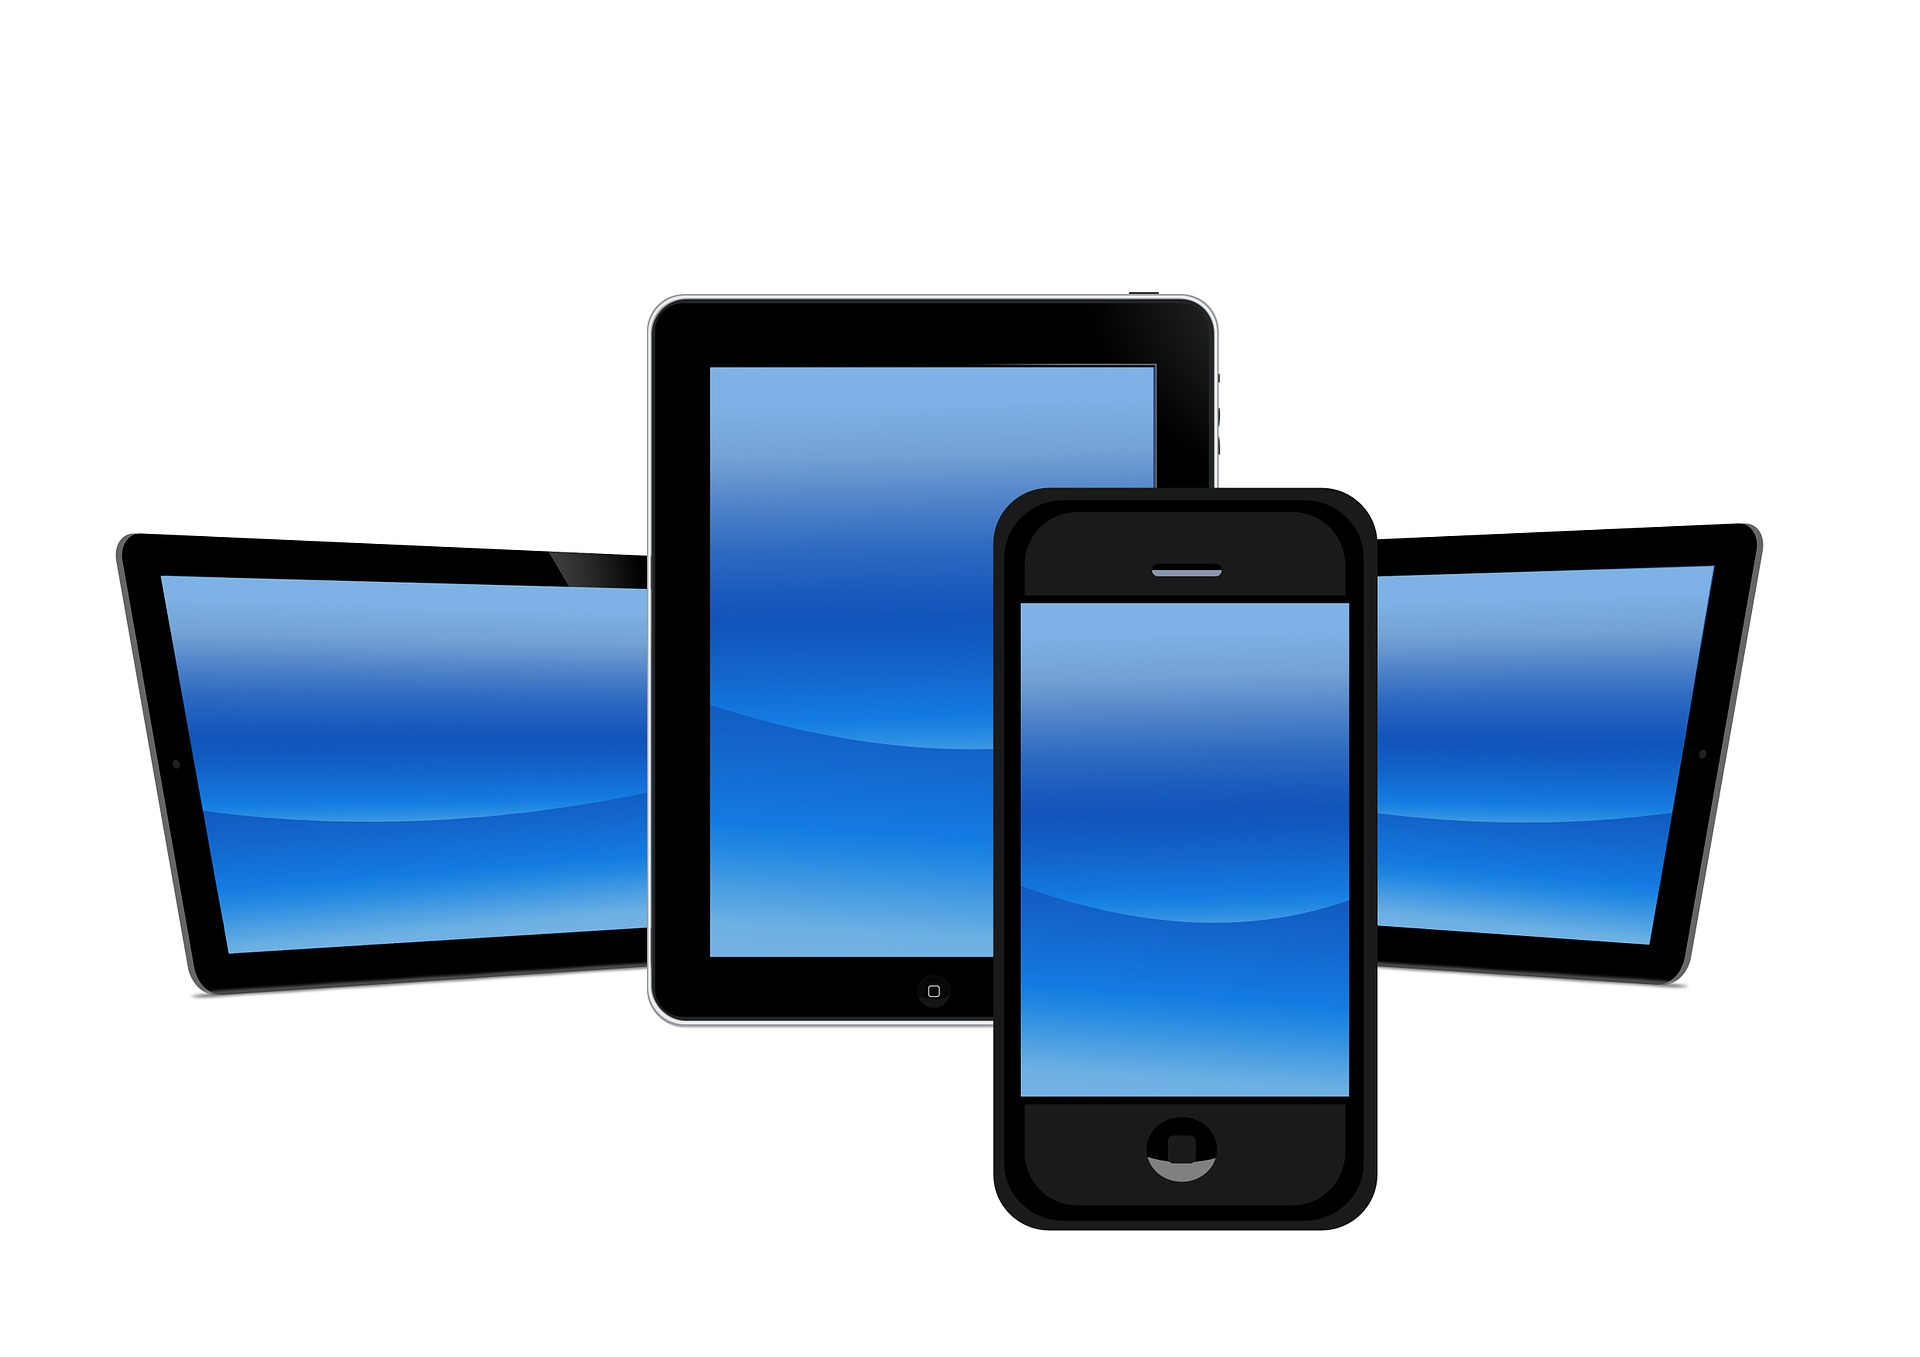
\includegraphics[scale=0.04]{images/mobile.jpg}
      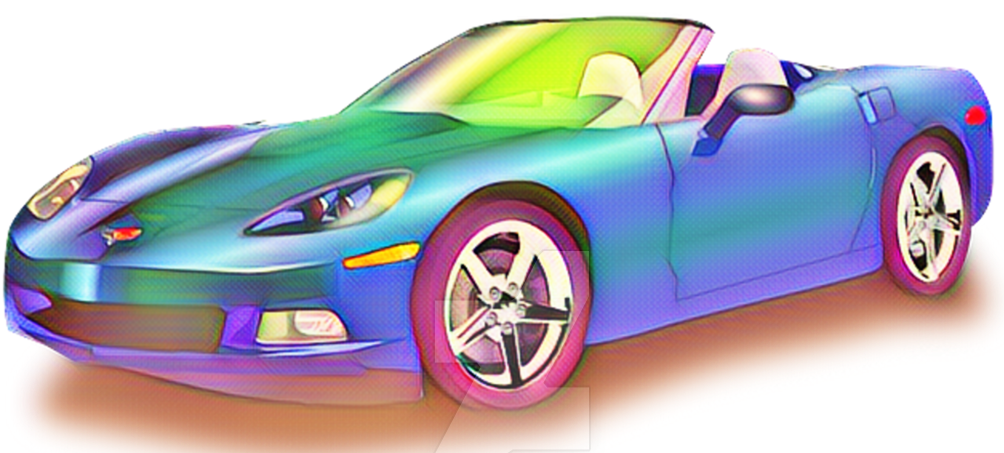
\includegraphics[scale=0.4]{images/car.png}
      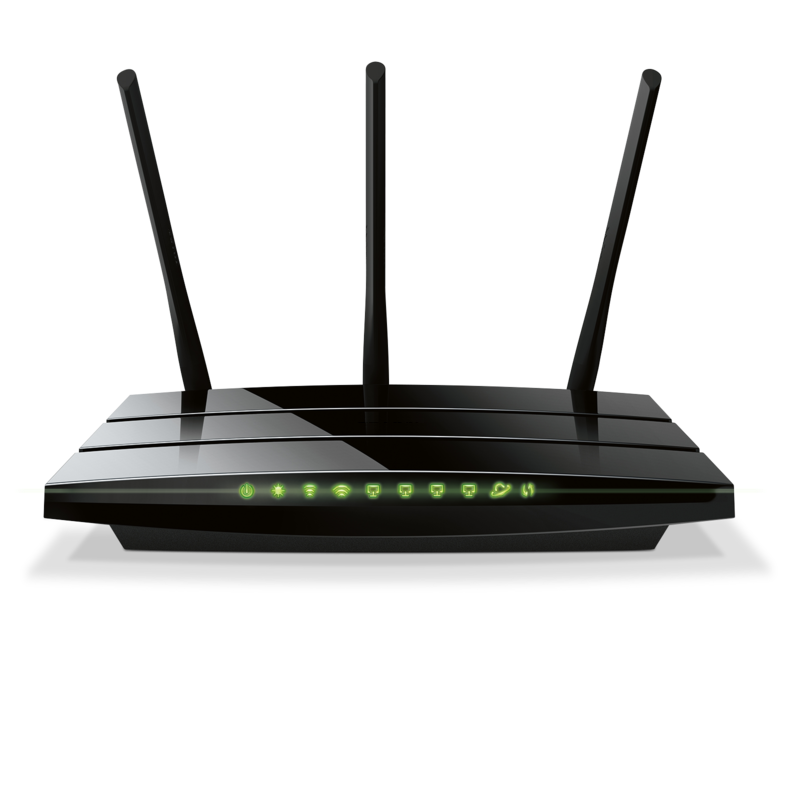
\includegraphics[scale=0.1]{images/router.png}
      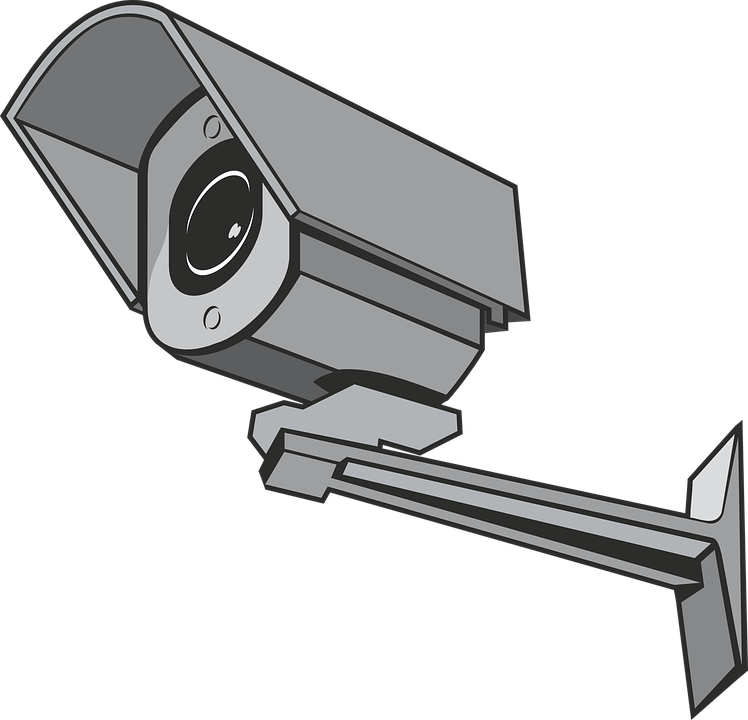
\includegraphics[scale=0.05]{images/surveillance-camera.png}
      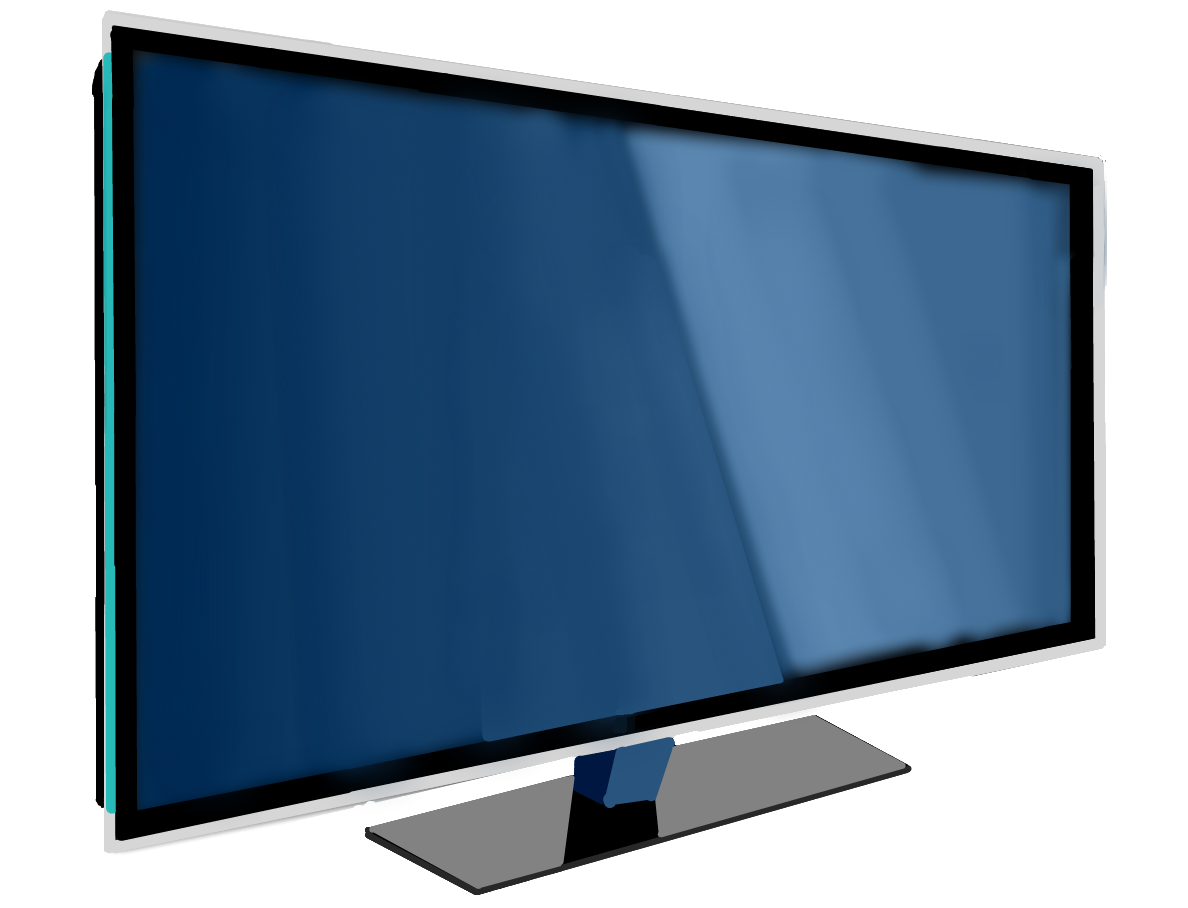
\includegraphics[scale=0.07]{images/tv.png}
      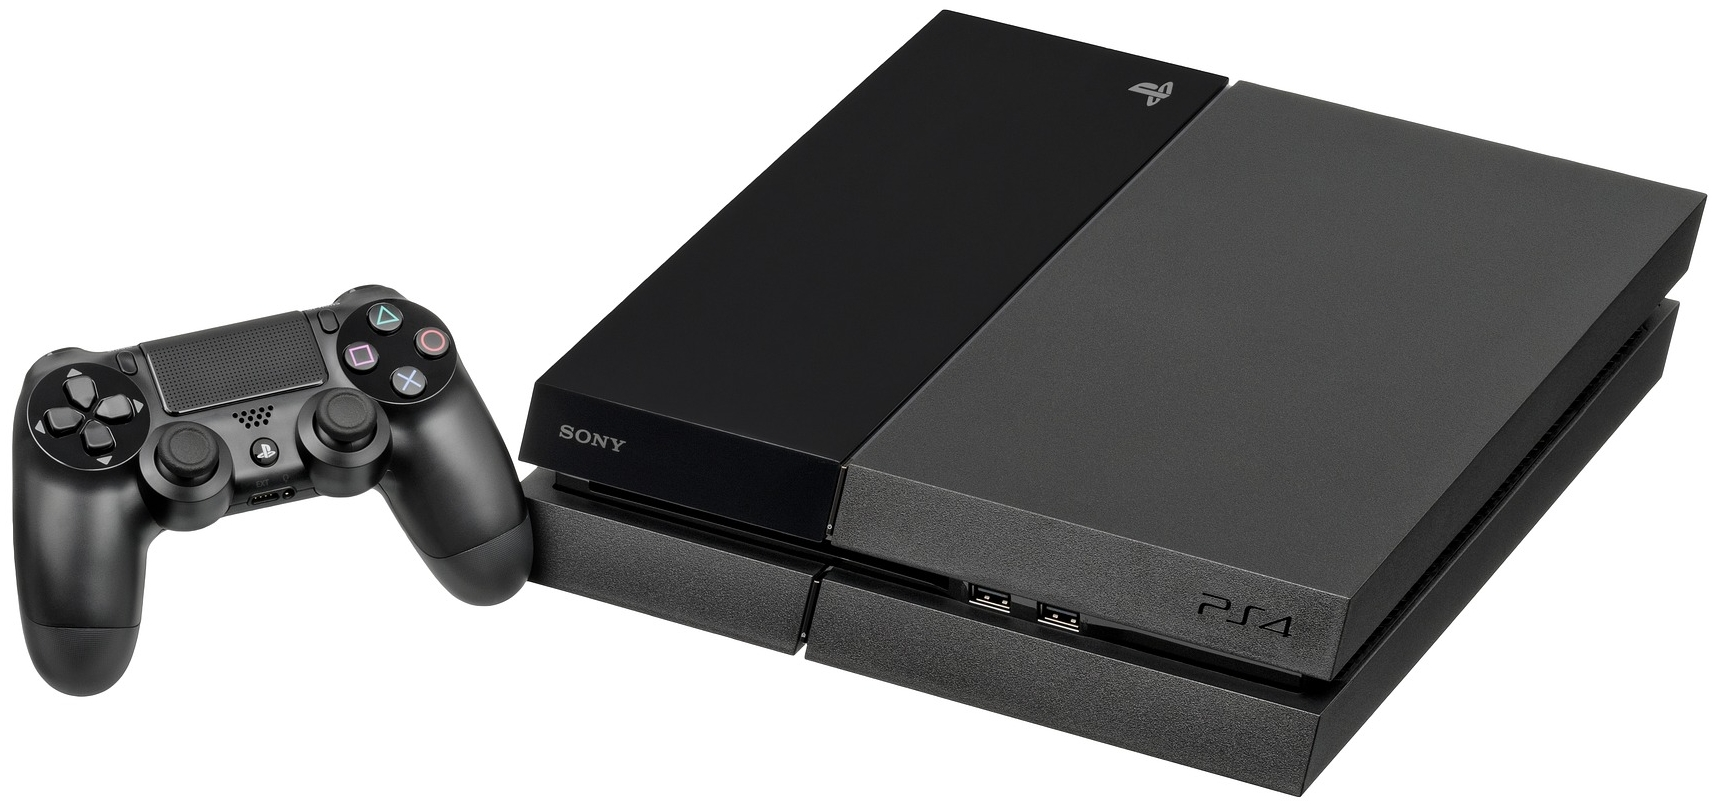
\includegraphics[scale=0.2]{images/game-console.jpg}
      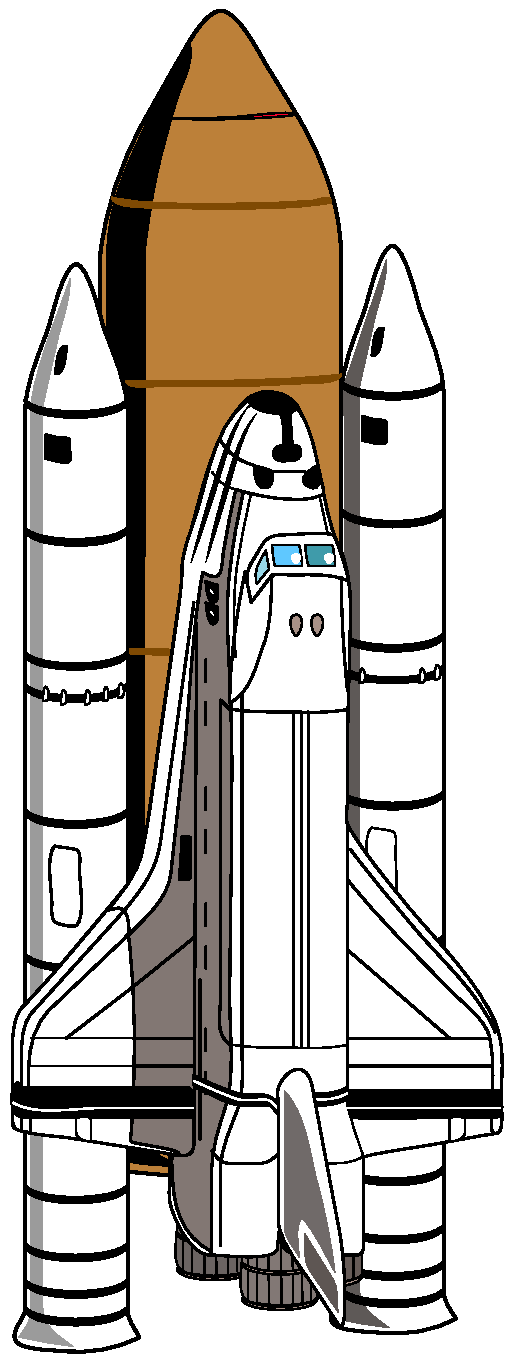
\includegraphics[scale=0.13]{images/shuttle.pdf}
      \centering
    \end{figure}
  \end{columns}
\end{frame}

\begin{frame}
  \frametitle{Android Rise}
  \vspace*{-2mm} % to reduce too much whitespace after figure block
    \begin{figure}
      \centering
      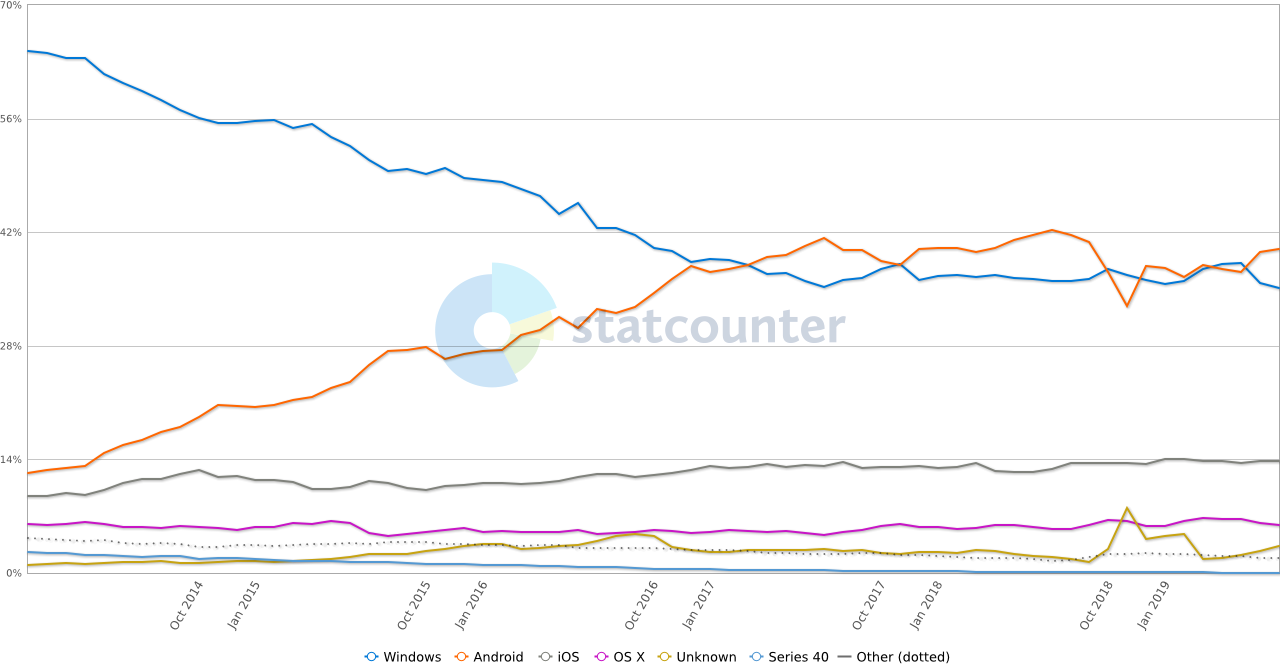
\includegraphics[scale=0.35]{images/os-stat.png}
      \vspace*{-2mm} % to reduce too much whitespace after figure block
      \caption{Operating System Market Share Worldwide}
    \end{figure}
  \vspace*{-12mm} % to reduce too much whitespace after figure block
\end{frame}

\begin{frame}
  \frametitle{Automotive Market Size}
    \begin{figure}
      \centering
      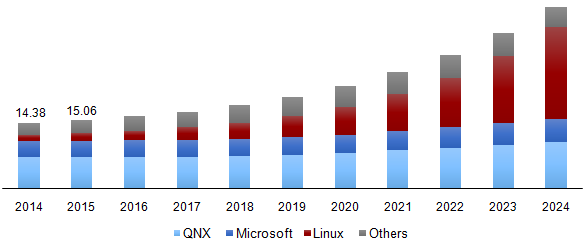
\includegraphics[scale=0.6]{images/automotive-market.png}
      \caption{Global automotive infotainment market, by operating system;
               \newline (2014 - 2024, USD Billion)}
    \end{figure}
    Source: \href{https://www.hexaresearch.com}{https://www.hexaresearch.com}
\end{frame}

\begin{frame}
  \frametitle{IoT Market Size}
    \begin{figure}
      \centering
      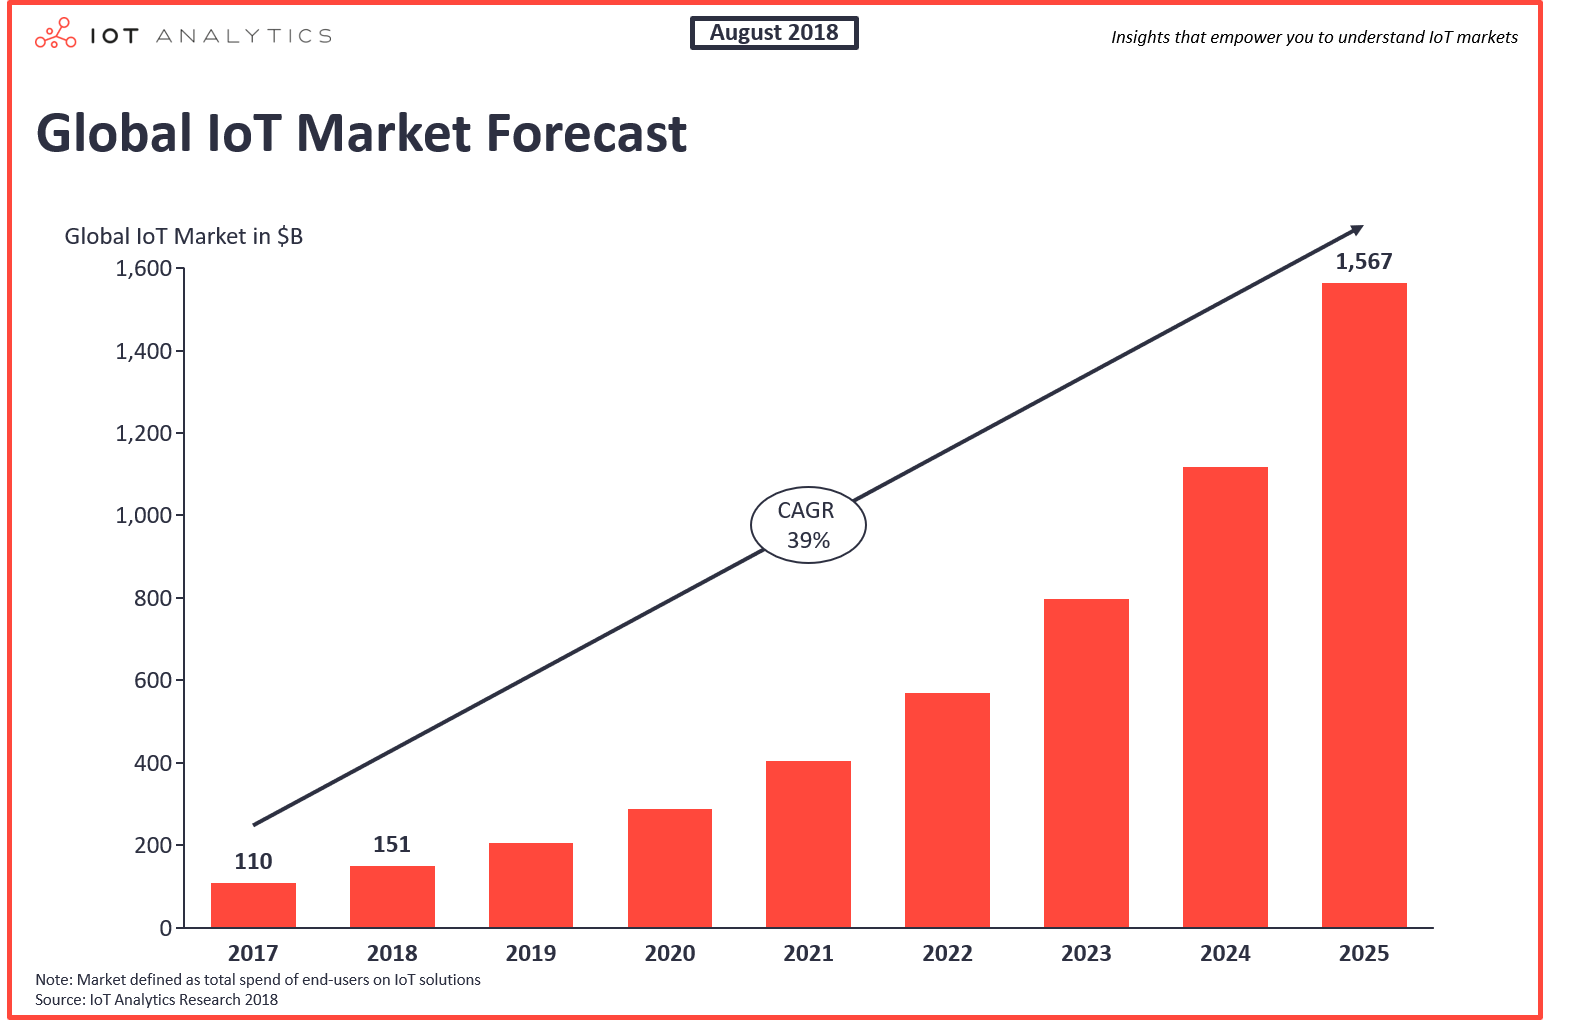
\includegraphics[scale=0.15]{images/iot1.png}
    \end{figure}
    Source: \href{https://iot-analytics.com}{https://iot-analytics.com}
\end{frame}

\begin{frame}
  \frametitle{IoT Number of Devices}
    \begin{figure}
      \centering
      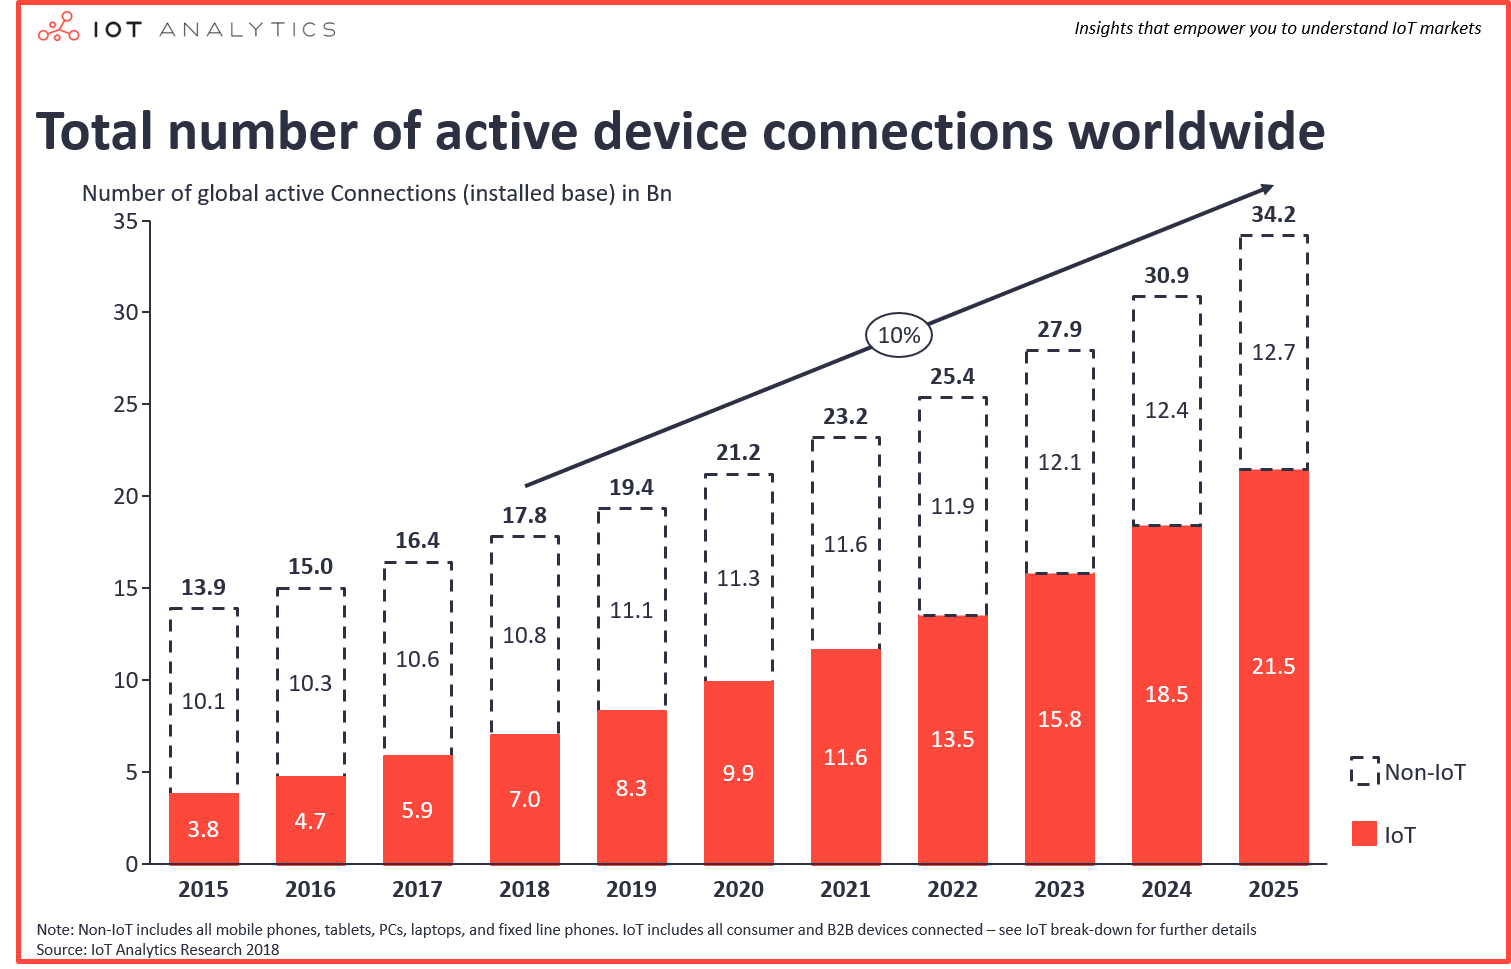
\includegraphics[scale=0.16]{images/iot2.png}
    \end{figure}
    Source: \href{https://iot-analytics.com}{https://iot-analytics.com}
\end{frame}

\begin{frame}
  \frametitle{How Linux kernel fits in?}
  \begin{columns}
    \column{0.5\textwidth}
    \textbf{Good fit for embedded:}
  \begin{itemize}
    \item Open-source (eases the collaboration)
    \item Supports a lot of architectures
    \item A lot of infrastructure exists (bootloaders, RootFS's, dev tools)
    \item Already widely used in Embedded world
  \end{itemize}

  \pause
    \column{0.5\textwidth}
  \textbf{Recent developments:}
  \begin{itemize}
    \item Reducing the kernel footprint (Nicolas Pitre)
    \item \texttt{PREEMPT\_RT} is being merged
    \item Xen
    \item OpenDataPlane vs DPDK
    \item RISC-V support
    \item Android kernel is mostly upstreamed now
  \end{itemize}
  \end{columns}
\end{frame}

\begin{frame}
  \frametitle{Embedded Linux Kernel Tasks}
  \begin{itemize}
    \item Board bring-up (porting the kernel to a new board)
    \item Writing the drivers and device tree
    \item Migrating downstream kernel to a new version
    \item Bug fixing
    \item Boot time optimization
    \item Upstreaming
    \item Related work: bootloader, rootfs, hardware debugging
  \end{itemize}
\end{frame}

\begin{frame}
  \frametitle{My Experience}
  \begin{itemize}
    \item Implementing the driver for automotive radio chip
    \item NOR flash support (XIP boot)
    \item Updating/upstreaming MAX732x driver
    \item Adopting upstream kernel VPN in Android kernel
    \item Fixing VPN protocols in kernel
    \item Implementing Android features (fastboot, boot flow, etc)
  \end{itemize}
\end{frame}

\section{Overture: Course Embedded Part}

\begin{frame}
  \frametitle{Embedded Programming}
  \begin{columns}
    \column{0.5\textwidth}
      Differences from regular system:
      \begin{itemize}
        \item Cross-compiling
        \item Flashing
        \item Serial console
        \item Testing concerns
        \item Working with hardware
        \item Non discoverable buses on board (device tree, platform drivers)
      \end{itemize}
    \column{0.5\textwidth}
      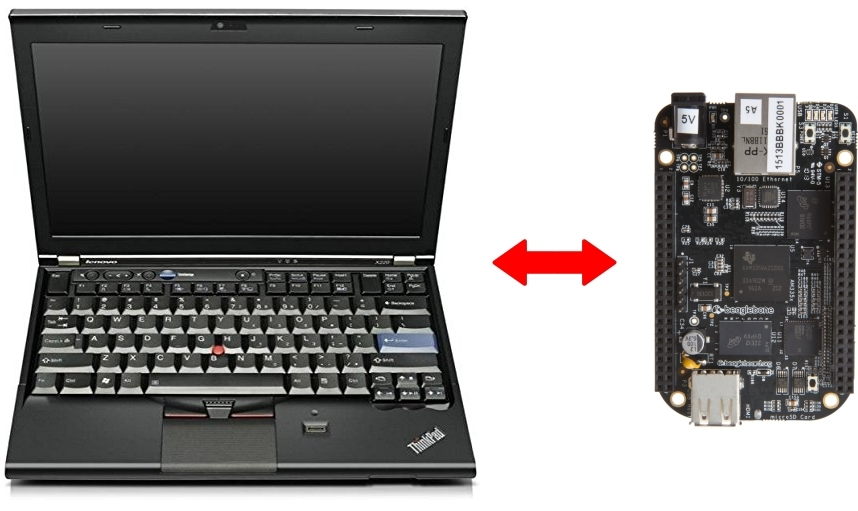
\includegraphics[scale=0.27]{images/host-target.jpg}
  \end{columns}
\end{frame}

\begin{frame}
  \frametitle{BeagleBone Black}
  \begin{center}
    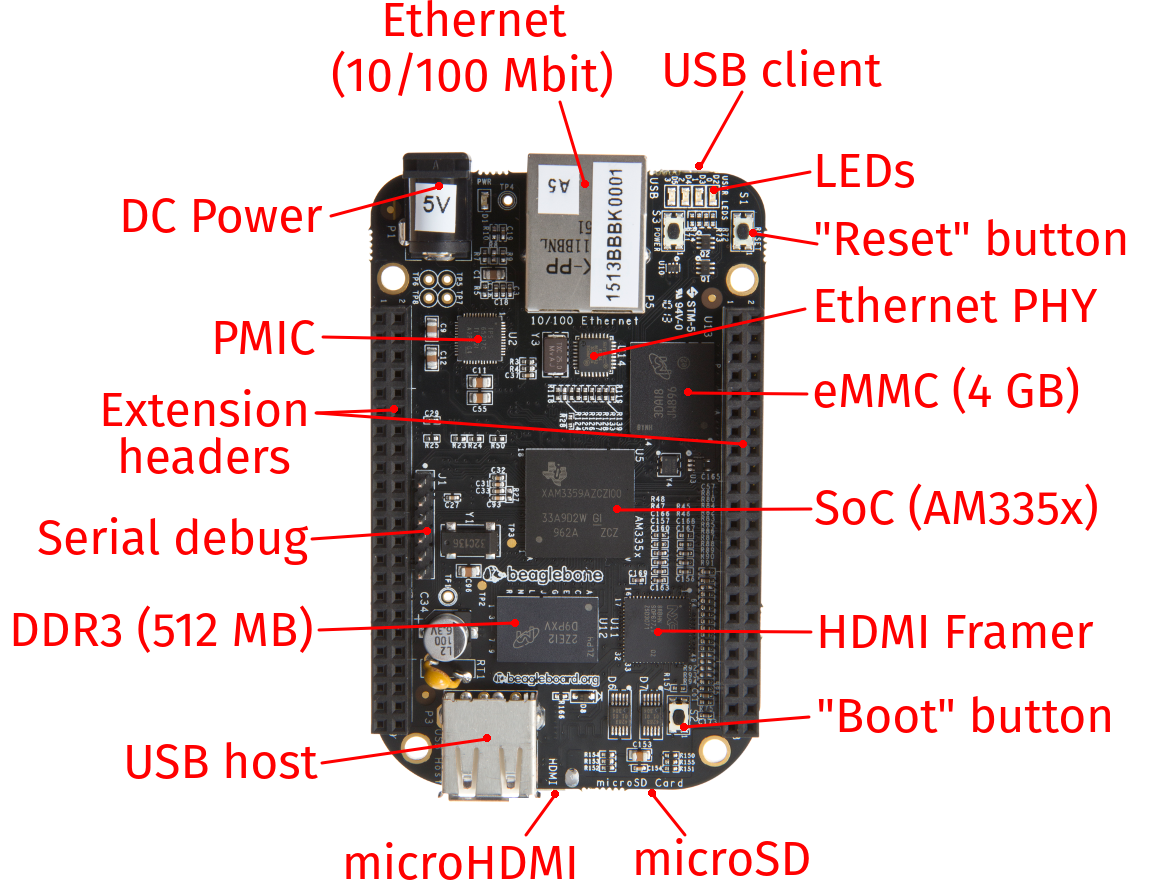
\includegraphics[scale=0.82]{images/bbb02.png}
  \end{center}
\end{frame}

\begin{frame}
  \frametitle{AM335x SoC}
  \begin{figure}
    \centering
    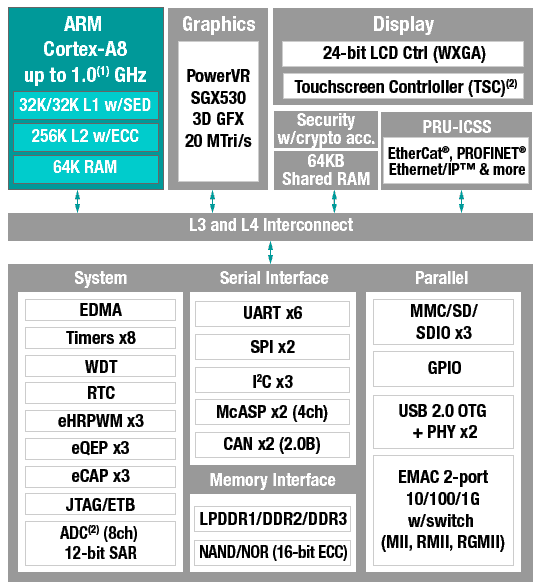
\includegraphics[scale=0.4]{images/am335x.png}
    \caption{AM335x Functional Diagram}
  \end{figure}
  \vspace*{-12mm} % to reduce too much whitespace after figure block
\end{frame}

\begin{frame}
  \frametitle{BeagleBone Black: Pros and Cons}
  \begin{columns}[t]
    \column{0.5\textwidth}
    Pros:
    \begin{itemize}
    \item Open Hardware
      \begin{itemize}
      \item Public TRM
      \item Schematic
      \item PCB files
      \end{itemize}
    \item Supported in upstream
      \begin{itemize}
      \item Kernel
      \item U-Boot
      \end{itemize}
    \item Conventional ARM architecture
    \item Very popular
    \item Low cost (\$55)
    \end{itemize}

    \column{0.5\textwidth}
    Cons:
    \begin{itemize}
    \item Old 32-bit architecture
    \item Single core processor
    \item Android is not supported officially
    \item No WiFi
    \end{itemize}
  \end{columns}
\end{frame}

\begin{frame}
  \frametitle{Embedded Topics}
  \underline{We will cover next Embedded topics during the course:}
  \begin{columns}
    \column{0.5\textwidth}
      \begin{itemize}
        \item<1-> Building, flashing and booting
        \item<2-> Bootloader and rootfs
        \item<3-> Electronics basics
        \item<4-> SoC architecture
        \item<5-> Buses and protocols
        \item<6-> Connecting external devices
        \item<7-> Writing the drivers
        \item<8-> Device Tree
        \item<9-> Hardware debugging
      \end{itemize}
    \column{0.5\textwidth}
      \only<1>{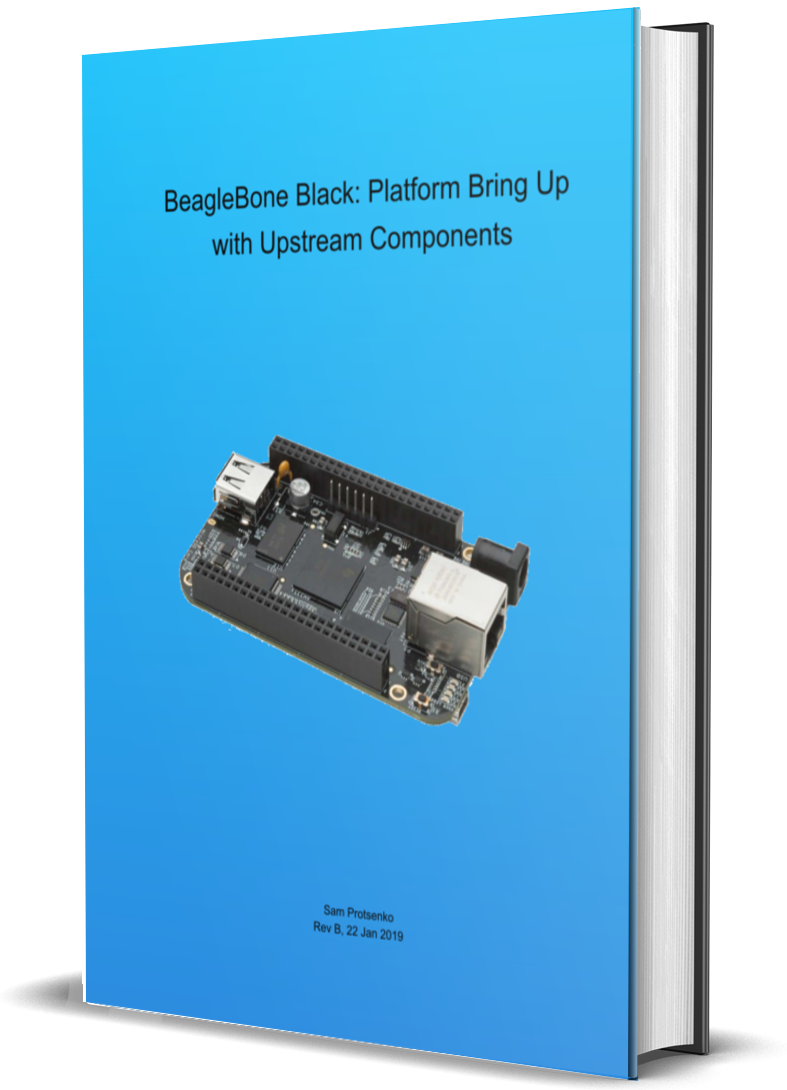
\includegraphics[scale=0.65]{images/metodichka.png}}
      \only<2>{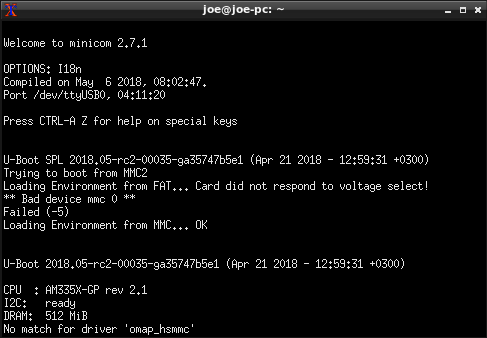
\includegraphics[scale=0.5]{images/minicom.png}}
      \only<3>{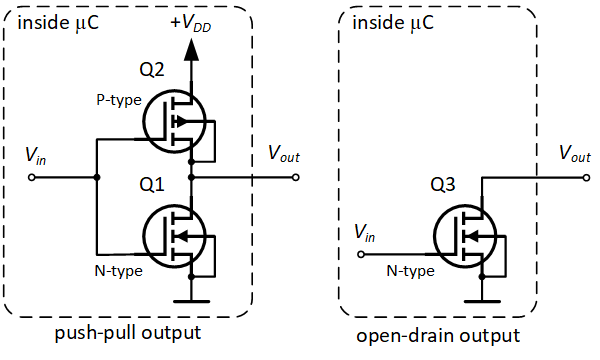
\includegraphics[scale=5.5]{images/outputs.png}}
      \only<4>{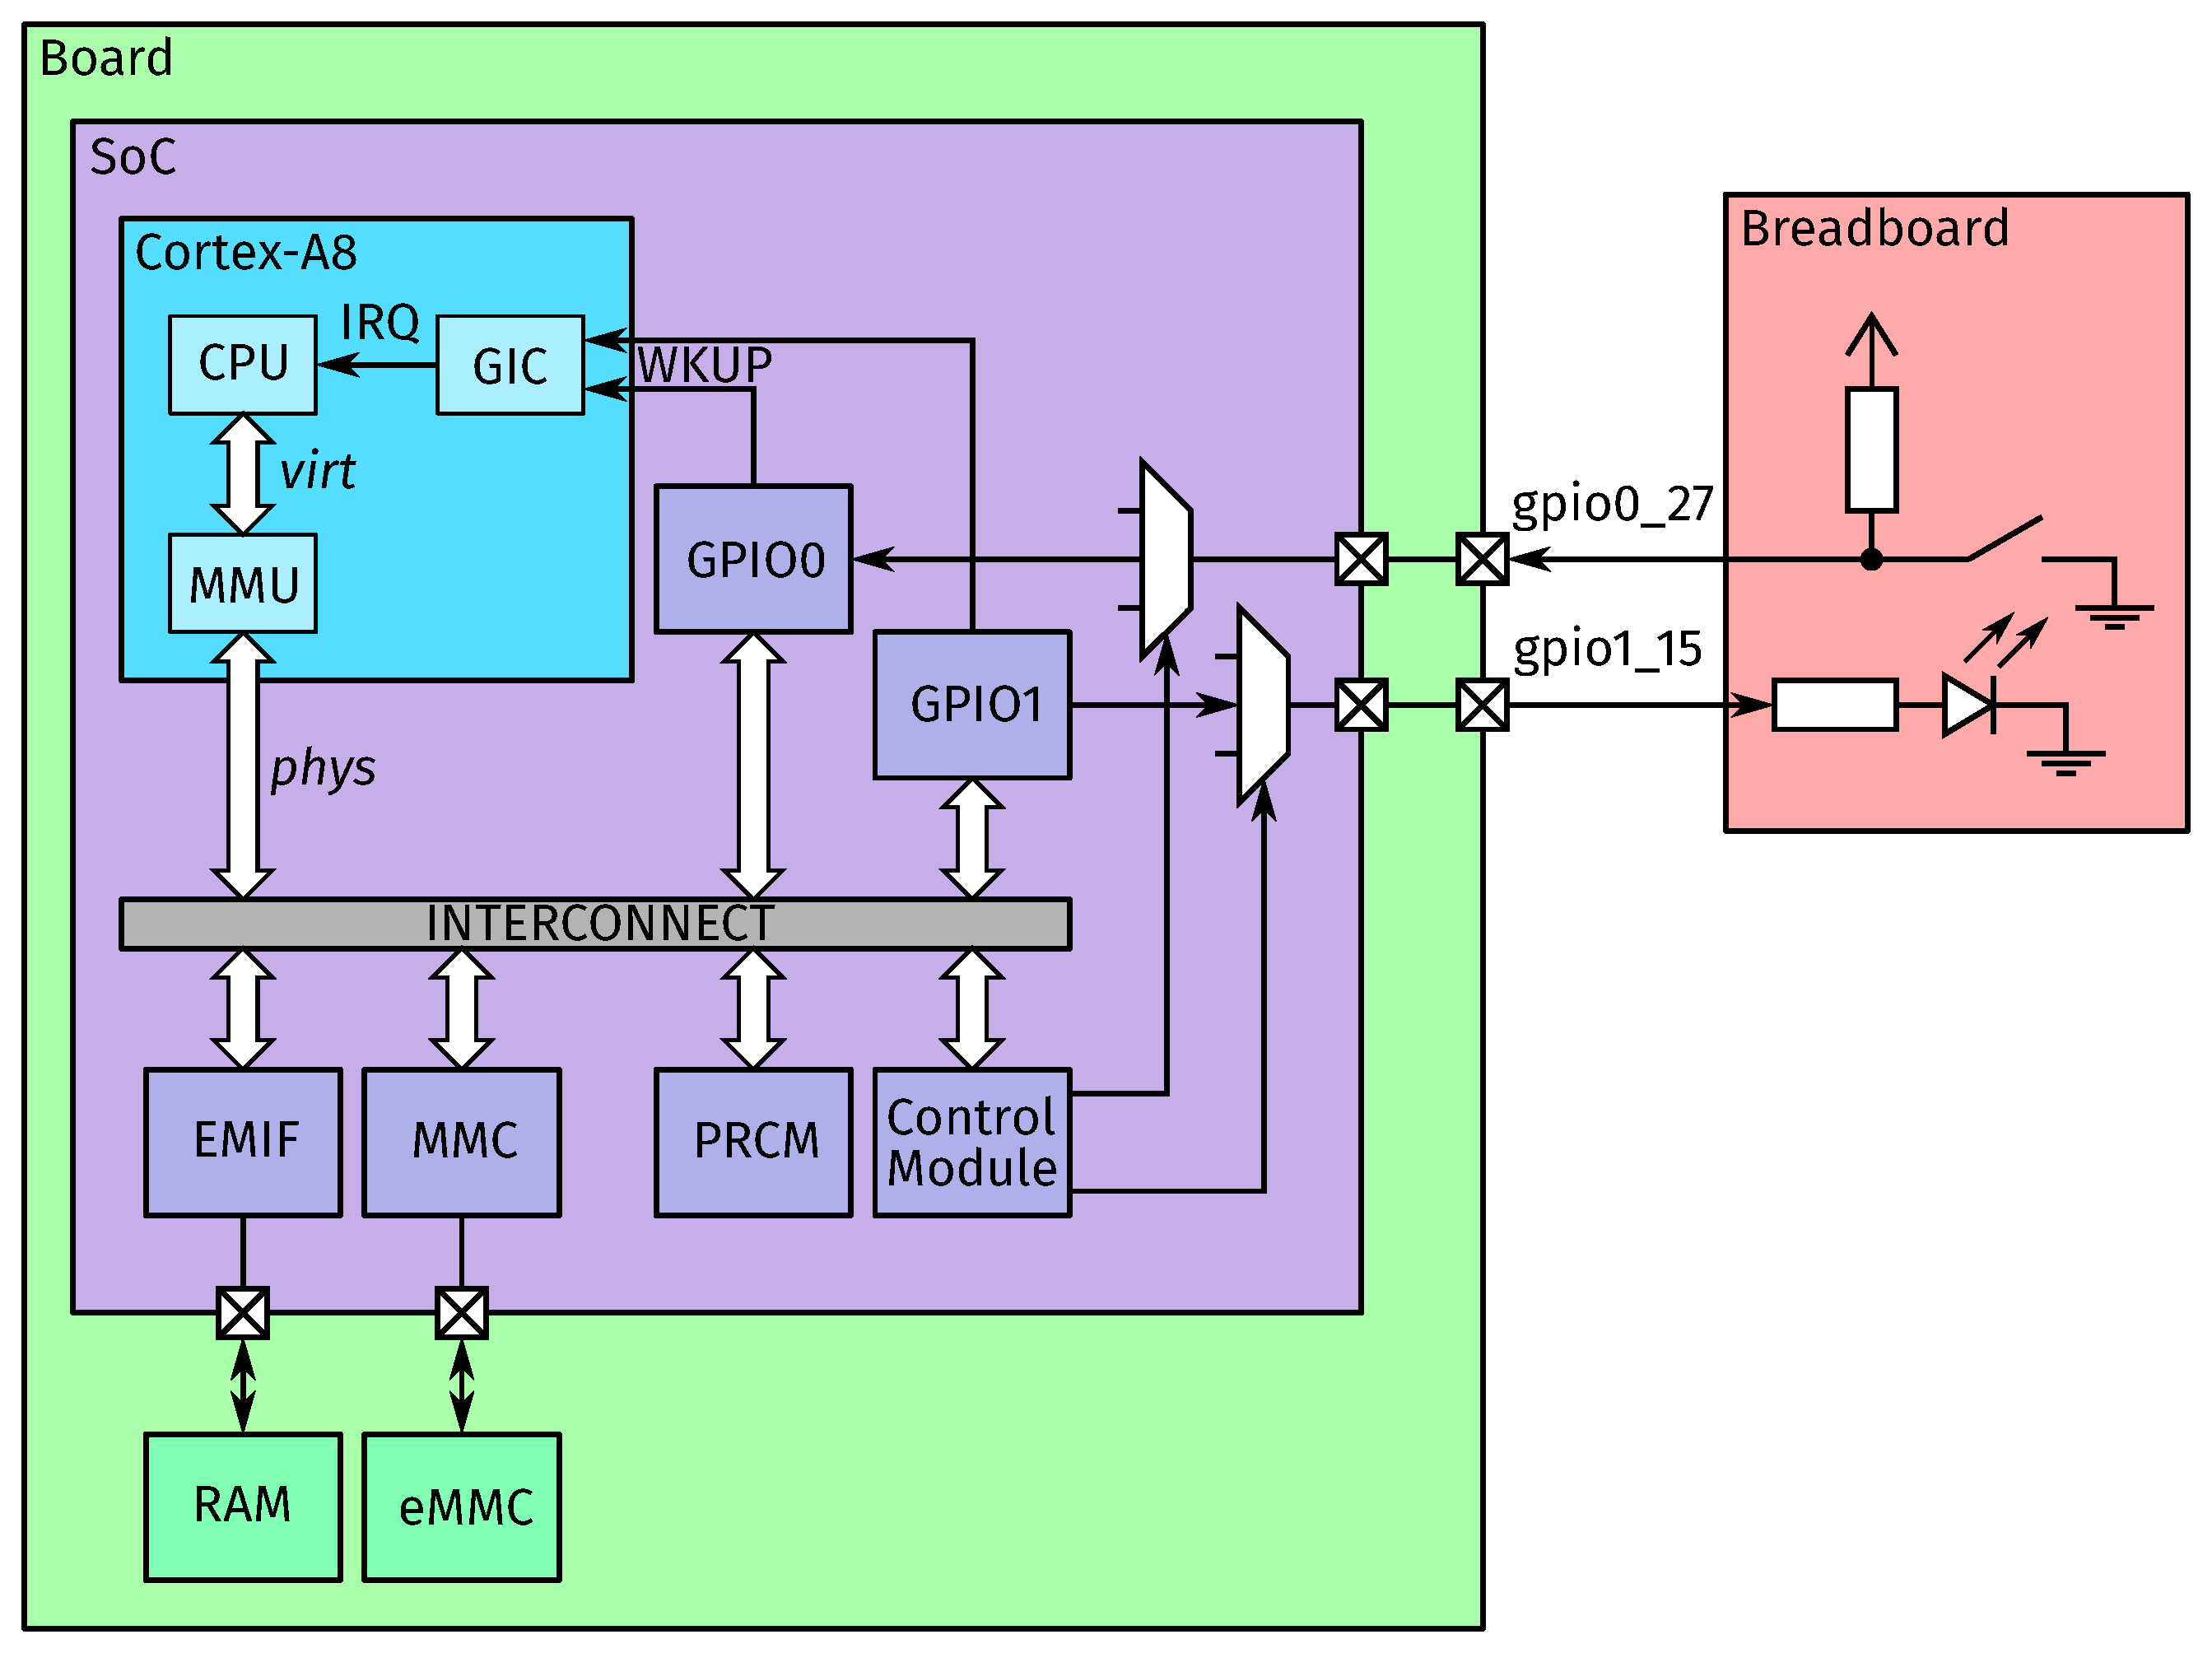
\includegraphics[scale=0.154]{images/architecture2.pdf}}
      \only<5>{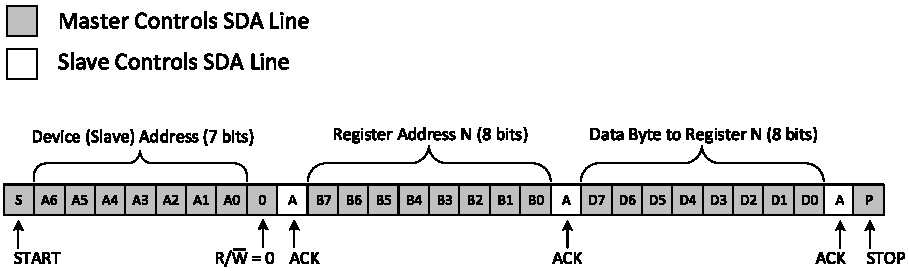
\includegraphics[scale=0.455]{images/i2c-write-reg.pdf}}
      \only<6>{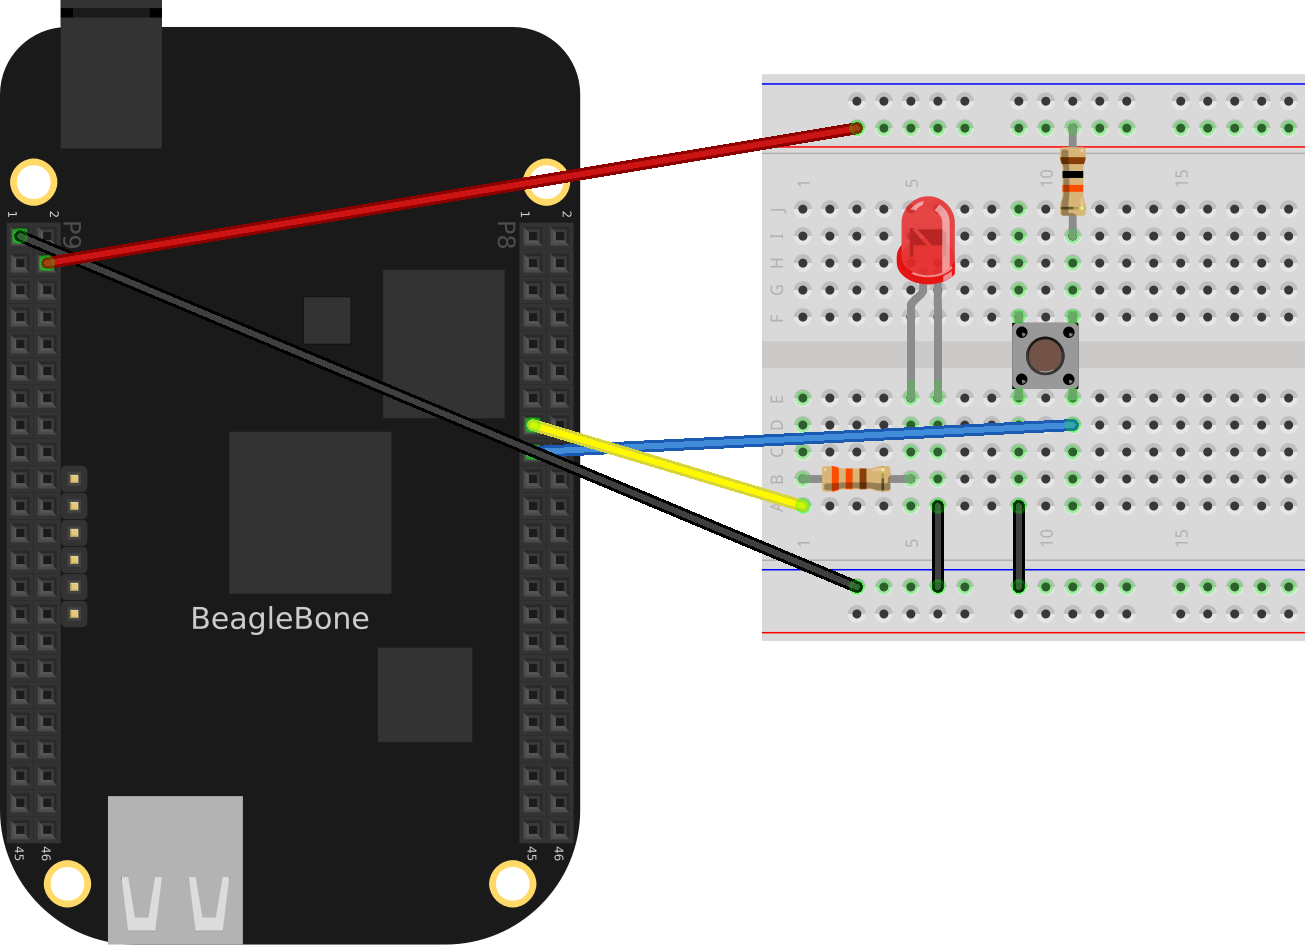
\includegraphics[scale=0.55]{images/lab1_bb.png}}
      \only<7>{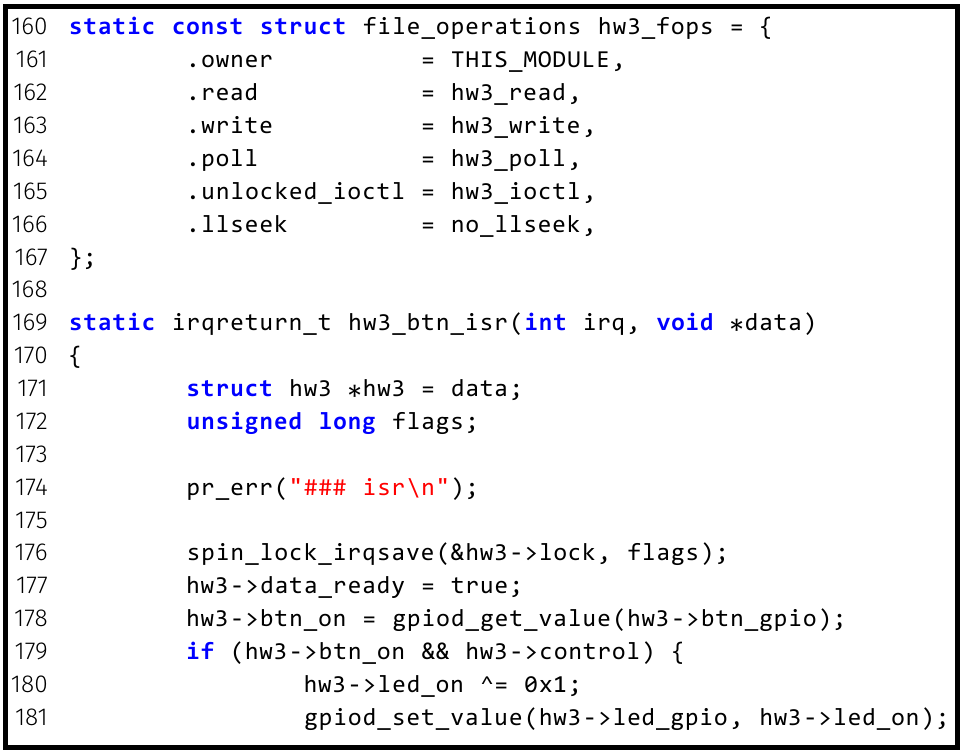
\includegraphics[scale=0.25]{images/driver.png}}
      \only<8>{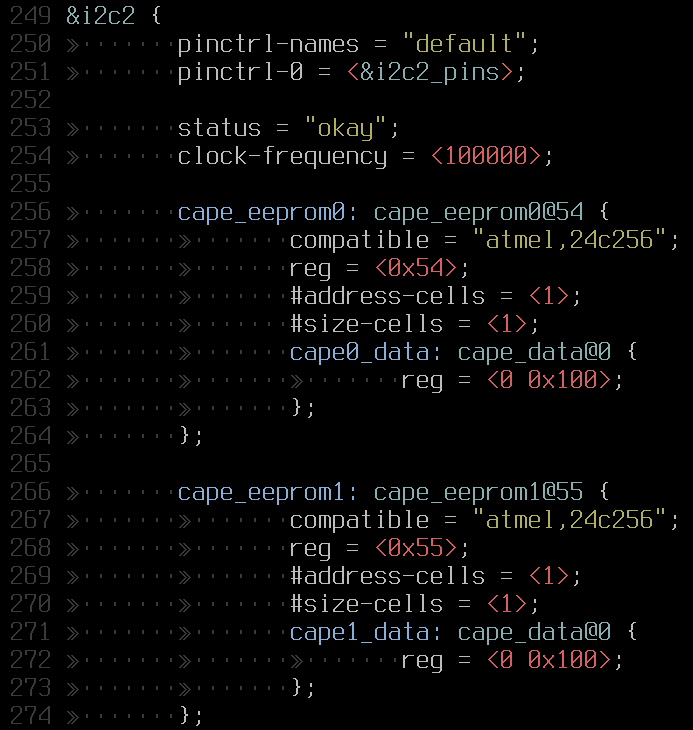
\includegraphics[scale=0.3]{images/device-tree.png}}
      \only<9>{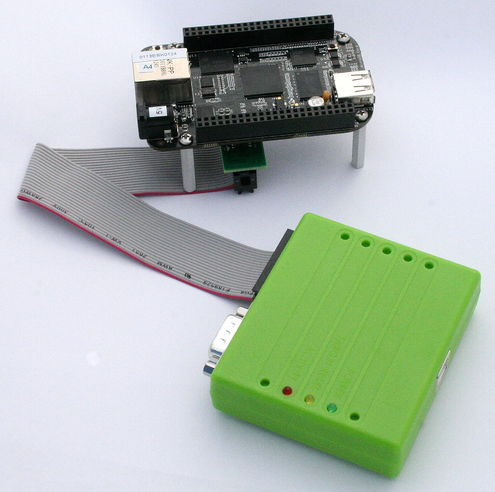
\includegraphics[scale=0.3]{images/bbb-and-flyswatter.jpg}}
      \vspace*{-12mm} % to reduce too much whitespace after figure block
  \end{columns}
\end{frame}

\begin{frame}
  \frametitle{What does it take?}
  \begin{itemize}

    \item We don't cover: C, Linux, Git, Makefiles
    \begin{itemize}
      \item ...learn along the way!
    \end{itemize}

    \pause
    \item 3 months
    \begin{itemize}
      \item ...is not too long!
    \end{itemize}

    \pause
    \item A lot of homework
    \begin{itemize}
      \item ...I encourage you to do even more hacking and test your ideas!
    \end{itemize}

    \pause
    \item Books: there are old ones and new ones; also LWN
    \begin{itemize}
      \item ...but \textit{practice makes perfect}!
    \end{itemize}

    \pause
    \item Working environment (IDE, toolchain, tools)
    \begin{itemize}
      \item ...people matter even more; Linux is all about community
    \end{itemize}
  \end{itemize}
\end{frame}

\section{UNIX/Linux History}

\begin{frame}
  \frametitle{2019: The Anniversaries}
  \begin{columns}
    \column{0.5\textwidth}
  \begin{itemize}
    \item 25 years: Linux kernel v1.0
    \item 30 years: WWW
    \item 50 years:
    \begin{itemize}
      \item UNIX
      \item Internet (ARPANET)
      \item People walking on the moon
      \item Linus Torvalds
    \end{itemize}
  \end{itemize}
    \column{0.5\textwidth}
      \pause
      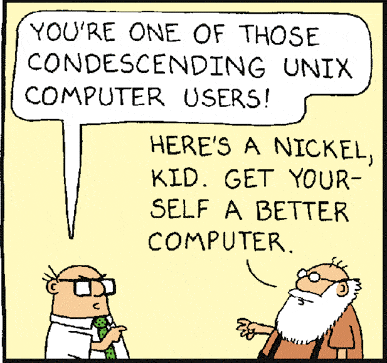
\includegraphics[scale=0.5]{images/nickel.png}
  \end{columns}

  \textit{(Credits: Maddog presentation at FOSDEM 2019)}
\end{frame}

\begin{frame}
  \frametitle{UNIX}
    \begin{quotation}
``...When BTL withdrew from the project, they needed to rewrite an OS in order
to play space war on another smaller machine (a DEC PDP-7 with 4K memory
for user programs). The result was a system which a punning colleague
called UNICS (UNiplexed Information and Computing Service) -- an
`emasculated Multics'; no one recalls whose idea the change to UNIX was.''
    \end{quotation}
    \vspace*{-5mm} % to reduce too much whitespace after figure block
    \begin{figure}
      \centering
      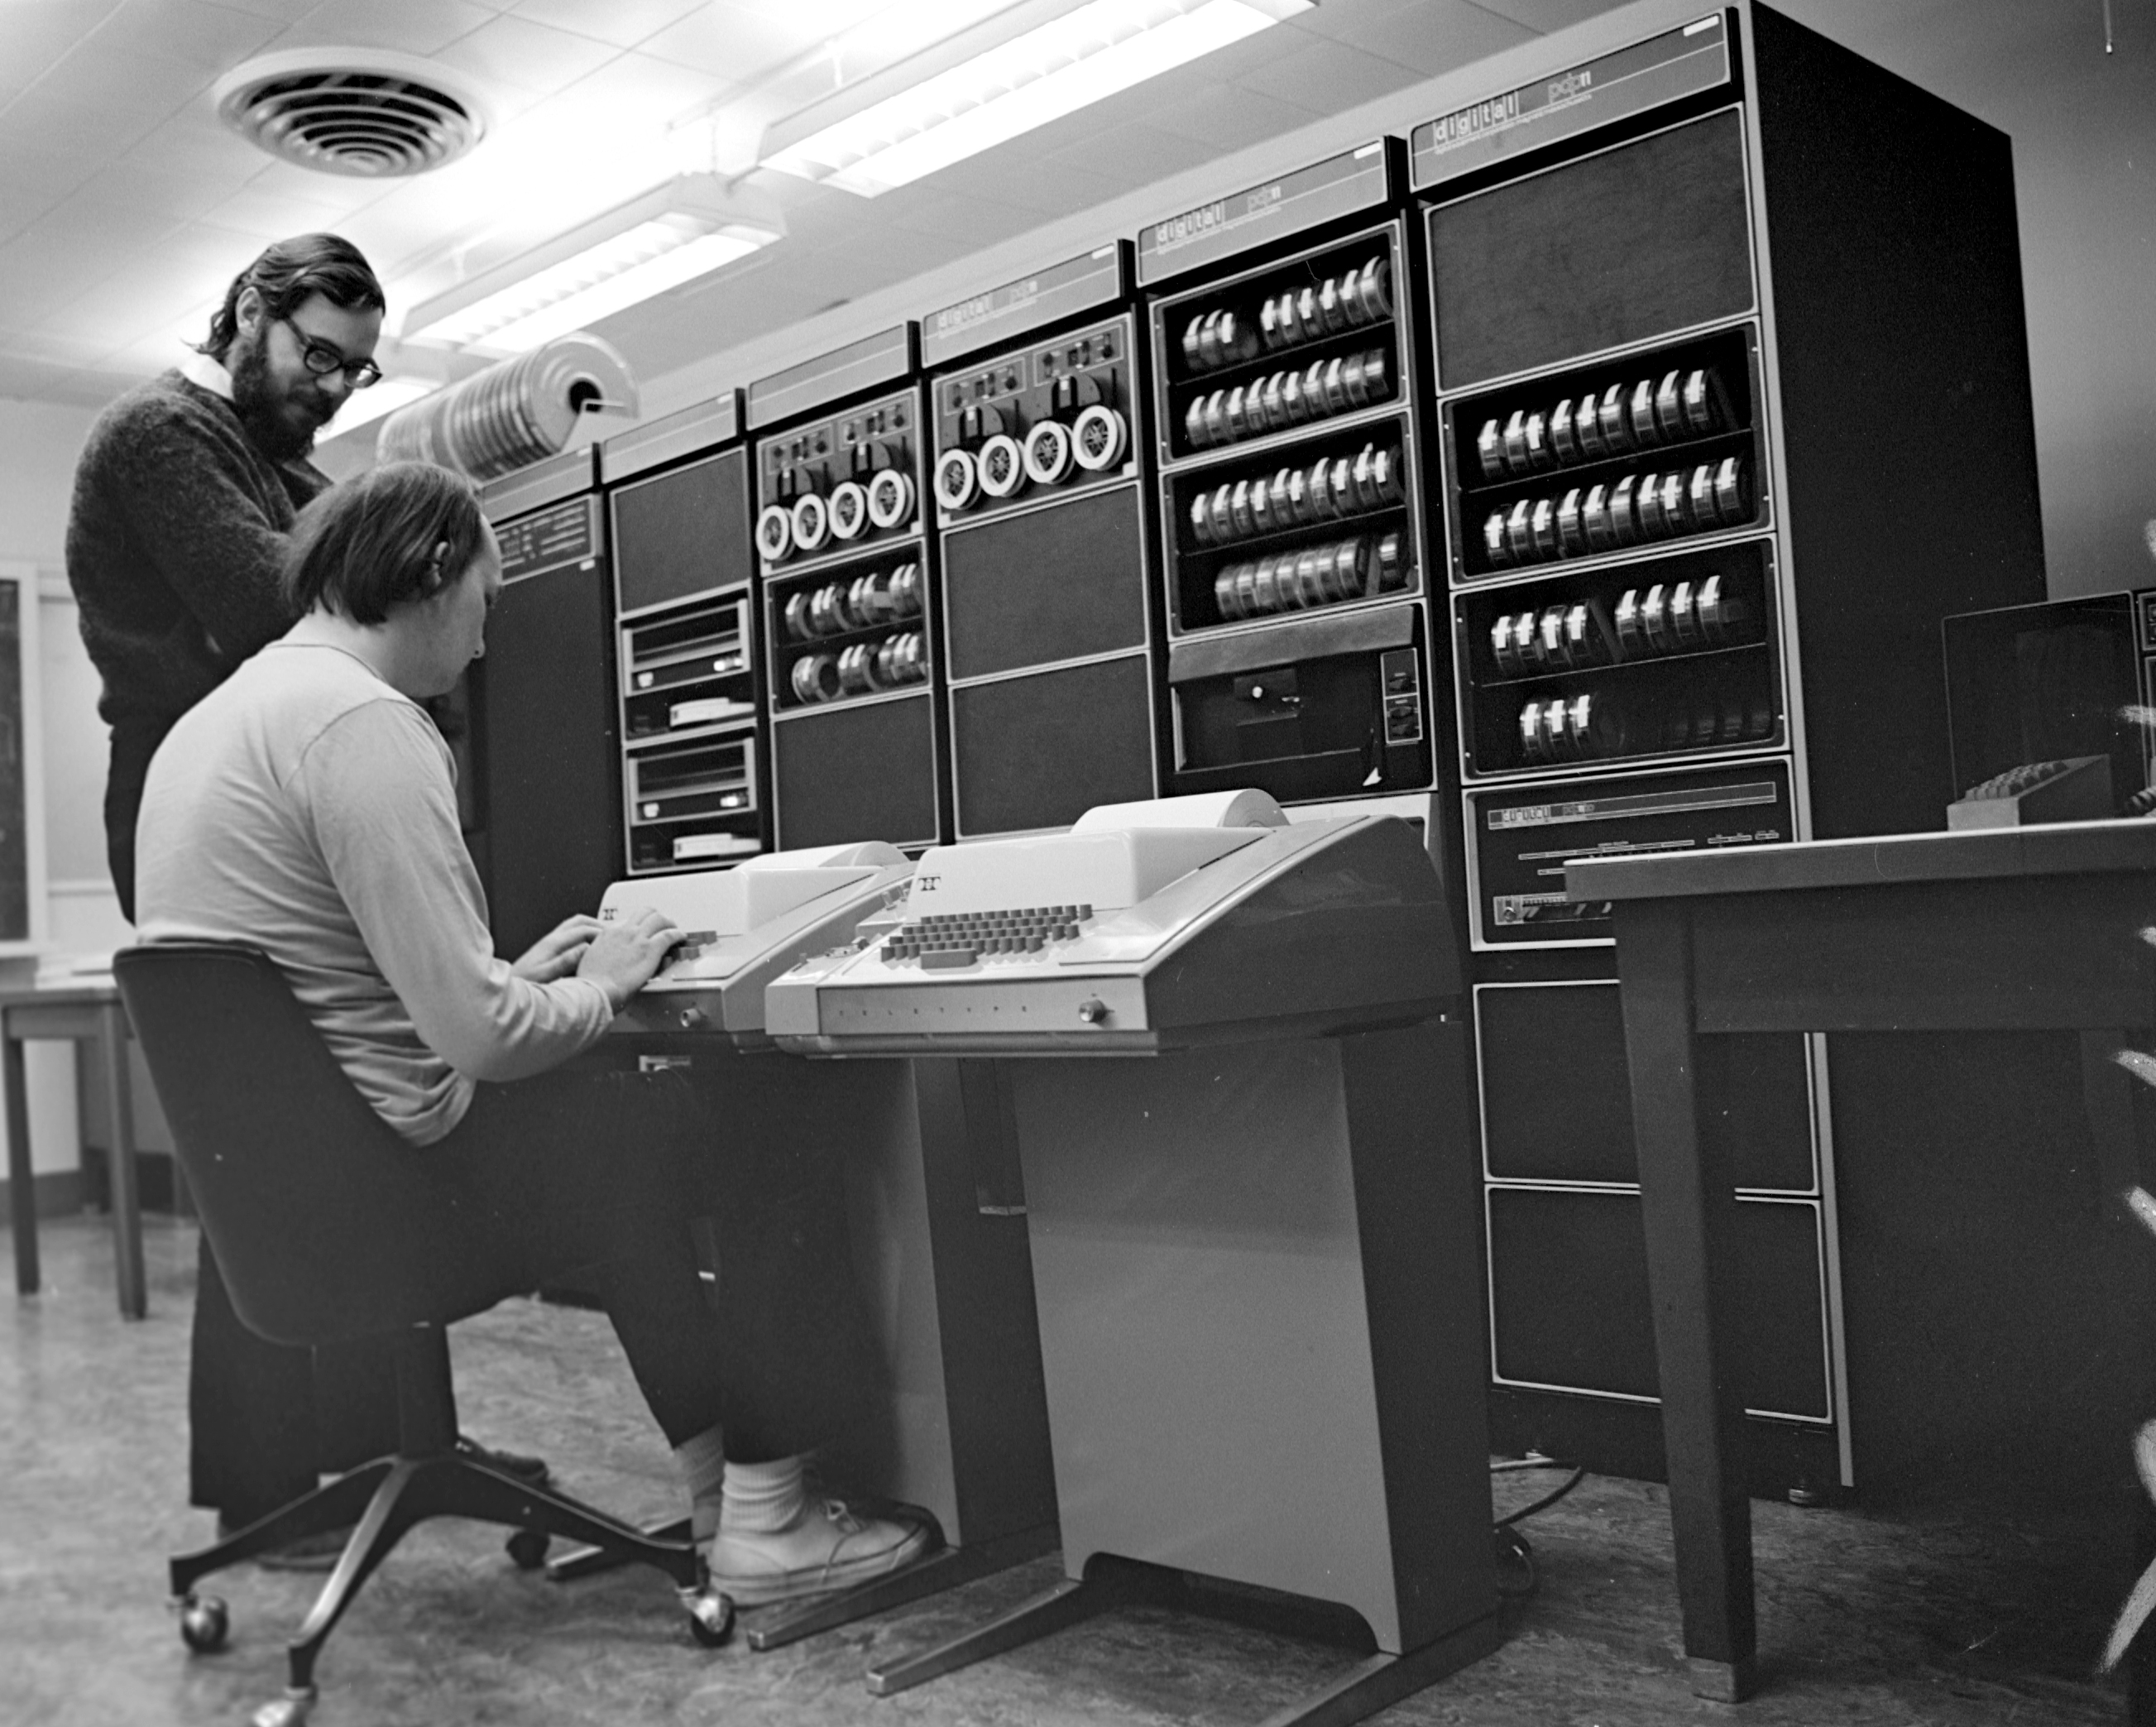
\includegraphics[scale=0.8]{images/ken-and-dennis.jpg}
    \end{figure}
    \vspace*{-12mm} % to reduce too much whitespace after figure block
\end{frame}

\begin{frame}
  \frametitle{UNIX (cont'd)}
  \begin{itemize}
    \item 1969: \textsc{UNIX} development started (PDP-7)
    \item 1971: V1, written in assembler (PDP-11/20)
    \item 1973: \textbf{V4 was re-written in C}
    \item 1975: V6 was available outside of Bell Labs (basis for BSD)
    \item 1979: V7: K\&R C, Bourne shell; ported to VAX (32-bit); kernel is only 40 KiB!
  \end{itemize}
\end{frame}

\begin{frame}
  \frametitle{GNU/Linux}
  \begin{itemize}
    \item 1984: \textsc{GNU} is not \textsc{UNIX}
    \item 1991: \textsc{Linux} v0.01
    \item 1994: \textsc{Linux} v1.0
    \item 2005: \textbf{First Git release}
  \end{itemize}
  \vspace*{5mm}
  \begin{quotation}
    ``Hello everybody out there using minix -
    I'm doing a (free) operating system (just a hobby, won't be big and
    professional like gnu) for 386(486) AT clones. This has been brewing
    since april, and is starting to get ready.''
  \end{quotation}
\end{frame}

\begin{frame}
  \frametitle{Linux Development Process}
    \begin{figure}
      \centering
      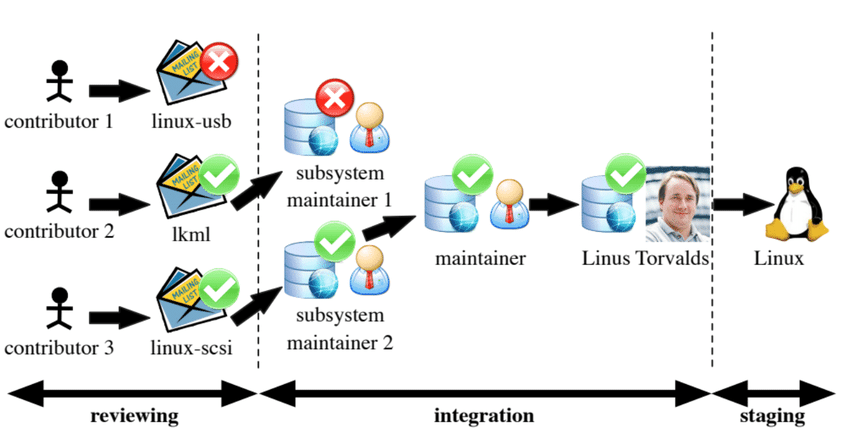
\includegraphics[scale=0.4]{images/linux-dev.png}
    \end{figure}
\end{frame}

\section*{References}

\begin{frame}
  \frametitle{References}
  \begin{thebibliography}{}
  \setbeamertemplate{bibliography item}[book]
    \bibitem{Cathedral1999}
      Eric S. Raymond.
      \newblock \emph{The Cathedral and the Bazaar}.
    \bibitem{Soul1981}
      Tracy Kidder.
      \newblock \emph{The Soul of a New Machine}.
    \bibitem{Hackers2010}
      Steven Levy.
     \newblock \emph{Hackers: Heroes of the Computer Revolution}, 25th
               Anniversary Edition.
  \end{thebibliography}
\end{frame}

\begin{frame}[standout]
  Thank you! \\
  \vspace{5mm}
	\href{mailto:semen.protsenko@globallogic.com}{\small \underline{semen.protsenko@globallogic.com}}
\end{frame}

\end{document}
